\usepackage[
  paperwidth=450.6bp,
  paperheight=707.6bp,
  margin=0bp,
  noheadfoot
]{geometry}
\usepackage{fontspec}
\usepackage{amsmath,amssymb}
\usepackage{graphicx}
\usepackage{xcolor}
\usepackage{tikz}
\usetikzlibrary{calc,shapes.geometric}
\usepackage[unicode,hidelinks]{hyperref}

\definecolor{illusiecover}{HTML}{FADC3C}
\definecolor{illusieeditionpaper}{HTML}{F4E7CE}
\definecolor{illusieeditionink}{HTML}{2C211B}
\definecolor{illusieeditionaccent}{HTML}{A94F2A}
\setmainfont{Latin Modern Roman}
\setsansfont{TeX Gyre Heros}
\DeclareMathSizes{7.1}{7.1}{5}{5}
\DeclareMathSizes{8.15}{8.15}{6}{5}
\DeclareMathSizes{6.45}{6}{5}{5}
\DeclareMathSizes{9.6}{10}{7}{5}
\DeclareMathSizes{9.3}{9}{7}{5}
\DeclareMathSizes{8.4}{8}{6}{5}
\DeclareMathSizes{7.8}{8}{6}{5}
\DeclareMathSizes{7.2}{7}{5}{5}
\DeclareMathSizes{6.2}{6}{5}{5}
\DeclareMathSizes{10.8}{10}{7}{5}
\DeclareMathSizes{10}{10}{7}{5}
\DeclareMathSizes{9.5}{9}{7}{5}
\DeclareMathSizes{8}{8}{6}{5}
\DeclareMathSizes{5.7}{6}{5}{5}
\DeclareMathSizes{9}{9}{6}{5}
\pagestyle{empty}
\setlength{\parindent}{0pt}

% Native TikZ reconstruction of the small Springer-Verlag cover device on
% LNM 239 physical p.1.  Authority crop: PDF points [105,545]-[165,640],
% rendered directly at 6000 dpi-equivalent.  The scan resolves the device as
% a chess knight above an ornamental oval SPRINGER/VERLAG medallion with a
% central S; scan noise and paper damage are not reproduced.

\newcommand{\IllusieSpringerMark}{%
  
\begin{tikzpicture}[
    baseline=(current bounding box.south),
    x=1cm,
    y=1cm,
    scale=0.58,
    every path/.style={line cap=round,line join=round}
  ]
    % Ornamental flanks and upper scrolls.
    \foreach \mirror in {-1,1}{%
      \begin{scope}[xscale=\mirror]
        \path[fill=black]
          (0.42,0.58)
          .. controls (0.72,0.68) and (0.92,0.55) .. (0.88,0.31)
          .. controls (0.85,0.15) and (0.72,0.15) .. (0.67,0.28)
          .. controls (0.62,0.40) and (0.72,0.46) .. (0.78,0.38)
          .. controls (0.86,0.26) and (0.78,0.08) .. (0.69,0.02)
          .. controls (0.88,-0.20) and (0.89,-0.65) .. (0.75,-0.98)
          .. controls (0.68,-1.13) and (0.58,-1.18) .. (0.52,-1.04)
          .. controls (0.46,-0.88) and (0.52,-0.64) .. (0.57,-0.48)
          .. controls (0.49,-0.55) and (0.43,-0.67) .. (0.39,-0.82)
          -- (0.31,-0.73)
          .. controls (0.38,-0.34) and (0.34,0.22) .. (0.42,0.58)
          -- cycle;
        \draw[illusiecover,line width=0.055cm]
          (0.72,0.31) .. controls (0.61,0.19) and (0.64,0.05) .. (0.74,-0.02);
        \draw[illusiecover,line width=0.045cm]
          (0.69,-0.16) .. controls (0.78,-0.39) and (0.74,-0.72) .. (0.60,-0.93);
        \draw[illusiecover,line width=0.035cm]
          (0.55,-0.08) .. controls (0.48,-0.28) and (0.49,-0.49) .. (0.56,-0.67);
        \path[fill=black]
          (0.36,0.63) .. controls (0.51,0.79) and (0.68,0.87) .. (0.77,0.77)
          .. controls (0.83,0.70) and (0.76,0.60) .. (0.66,0.63)
          .. controls (0.59,0.65) and (0.61,0.73) .. (0.67,0.71)
          .. controls (0.61,0.63) and (0.49,0.58) .. (0.36,0.63) -- cycle;
      \end{scope}%
    }

    % Lower ribbon, knot, and small terminal flourish.
    \path[fill=black]
      (-0.64,-0.96)
      .. controls (-0.76,-1.03) and (-0.79,-1.17) .. (-0.67,-1.25)
      .. controls (-0.53,-1.34) and (-0.40,-1.27) .. (-0.31,-1.17)
      .. controls (-0.20,-1.32) and (-0.09,-1.29) .. (0,-1.14)
      .. controls (0.09,-1.29) and (0.20,-1.32) .. (0.31,-1.17)
      .. controls (0.40,-1.27) and (0.53,-1.34) .. (0.67,-1.25)
      .. controls (0.79,-1.17) and (0.76,-1.03) .. (0.64,-0.96)
      .. controls (0.55,-0.91) and (0.50,-1.00) .. (0.58,-1.06)
      .. controls (0.48,-1.04) and (0.41,-0.99) .. (0.35,-0.91)
      .. controls (0.25,-1.07) and (0.13,-1.03) .. (0,-0.91)
      .. controls (-0.13,-1.03) and (-0.25,-1.07) .. (-0.35,-0.91)
      .. controls (-0.41,-0.99) and (-0.48,-1.04) .. (-0.58,-1.06)
      .. controls (-0.50,-1.00) and (-0.55,-0.91) .. (-0.64,-0.96)
      -- cycle;
    \path[fill=black]
      (-0.18,-1.18) -- (-0.12,-1.42) -- (-0.24,-1.50)
      -- (0,-1.55) -- (0.24,-1.50) -- (0.12,-1.42) -- (0.18,-1.18)
      -- cycle;
    \draw[illusiecover,line width=0.04cm]
      (-0.10,-1.31) -- (0,-1.37) -- (0.10,-1.31);
    \draw[illusiecover,line width=0.04cm]
      (-0.11,-1.42) -- (0,-1.47) -- (0.11,-1.42);

    % Oval publisher medallion.
    \path[fill=black] (0,-0.25) ellipse [x radius=0.69,y radius=0.88];
    \draw[illusiecover,line width=0.045cm]
      (0,-0.25) ellipse [x radius=0.62,y radius=0.80];
    \draw[illusiecover,line width=0.045cm]
      (0,-0.25) ellipse [x radius=0.45,y radius=0.62];

    % Ring lettering.  Each glyph is native text placed on the scanned oval.
    \foreach \a/\glyph in {151/S,132/P,113/R,94/I,75/N,56/G,37/E,18/R}{%
      \node[
        text=illusiecover,
        font=\sffamily\bfseries\fontsize{2.7}{2.7}\selectfont,
        rotate=\a-90,
        inner sep=0pt
      ] at ({0.535*cos(\a)},{-0.25+0.705*sin(\a)}) {\glyph};
    }
    \foreach \a/\glyph in {205/V,230/E,255/R,280/L,305/A,330/G}{%
      \node[
        text=illusiecover,
        font=\sffamily\bfseries\fontsize{2.7}{2.7}\selectfont,
        rotate=\a+90,
        inner sep=0pt
      ] at ({0.535*cos(\a)},{-0.25+0.705*sin(\a)}) {\glyph};
    }
    \fill[illusiecover] (-0.54,-0.25) circle (0.035);
    \fill[illusiecover] (0.54,-0.25) circle (0.035);

    % Central S, intentionally serifed as on the historical device.
    \node[
      text=illusiecover,
      font=\rmfamily\fontsize{18}{18}\selectfont,
      inner sep=0pt
    ] at (0,-0.25) {S};

    % Chess knight and its stepped base.
    \path[fill=black]
      (-0.31,0.54)
      .. controls (-0.28,0.72) and (-0.22,0.86) .. (-0.13,0.96)
      .. controls (-0.27,0.93) and (-0.42,0.91) .. (-0.51,1.01)
      .. controls (-0.57,1.08) and (-0.53,1.18) .. (-0.43,1.23)
      .. controls (-0.31,1.29) and (-0.25,1.38) .. (-0.28,1.51)
      -- (-0.20,1.45)
      -- (-0.12,1.62)
      -- (-0.03,1.47)
      .. controls (0.15,1.48) and (0.30,1.38) .. (0.34,1.19)
      .. controls (0.37,1.02) and (0.31,0.80) .. (0.20,0.65)
      -- (0.31,0.54)
      -- cycle;
    \path[fill=illusiecover]
      (-0.10,1.38)
      .. controls (-0.14,1.25) and (-0.23,1.14) .. (-0.37,1.07)
      .. controls (-0.25,1.05) and (-0.13,1.08) .. (-0.02,1.16)
      .. controls (-0.02,1.02) and (-0.11,0.89) .. (-0.22,0.75)
      .. controls (-0.08,0.82) and (0.04,0.95) .. (0.11,1.10)
      .. controls (0.16,1.21) and (0.14,1.33) .. (-0.10,1.38)
      -- cycle;
    \fill[illusiecover] (-0.21,1.29) circle (0.027);
    \draw[illusiecover,line width=0.035cm]
      (-0.42,1.10) .. controls (-0.34,1.08) and (-0.28,1.09) .. (-0.22,1.13);
    \draw[black,line width=0.055cm] (-0.30,0.61) -- (0.28,0.61);
    \draw[black,line width=0.055cm] (-0.24,0.55) -- (0.24,0.55);

    % Small heraldic bars joining knight and medallion.
    \path[fill=black]
      (-0.35,0.53) -- (0.35,0.53) -- (0.30,0.43) -- (-0.30,0.43) -- cycle;
    \draw[illusiecover,line width=0.035cm] (-0.22,0.49) -- (0.22,0.49);
  \end{tikzpicture}%
}

% LNM 239 physical p.2 is publisher matter whose source language is English.
% Direct authority: Volume I PDF physical page 2, broad review at 1100
% dpi-equivalent; the obscured manuscript line and 10 1/2-inch measurement
% were separately inspected at 5500 dpi-equivalent. No OCR was generated.

\newcommand{\IllusiePublisherPtwoUpperSource}{%
  This series aims to report new developments in mathematical research and
  teaching - quickly, informally and at a high level. The type of material
  considered for publication includes:\par
  \vspace{0.50em}
  \begin{tabular}{@{}r@{\hspace{0.45em}}p{0.90\linewidth}@{}}
    1. & Preliminary drafts of original papers and monographs\\[0.18em]
    2. & Lectures on a new field, or presenting a new angle on a classical field\\[0.18em]
    3. & Seminar work-outs\\[0.18em]
    4. & Reports of meetings, provided they are\\[-0.05em]
       & \hspace{0.75em}a) of exceptional interest or\\[-0.05em]
       & \hspace{0.75em}b) devoted to a single topic.
  \end{tabular}\par
  \vspace{0.75em}
  Texts which are out of print but still in demand may also be considered if
  they fall within these categories.\par
  \vspace{0.75em}
  The timeliness of a manuscript is more important than its form, which may be
  unfinished or tentative. Thus, in some instances, proofs may be merely
  outlined and results presented which have been or will later be published
  elsewhere.\par
  \vspace{0.75em}
  Manuscripts should comprise not less than 100 pages.\par
  \vspace{0.75em}
  Publication of \textit{Lecture Notes} is intended as a service to the
  international mathematical community, in that a commercial publisher,
  Springer-Verlag, can offer a wider distribution to documents which would
  otherwise have a restricted readership. Once published and copyrighted,
  they can be documented in the scientific literature. -\par
  \vspace{0.75em}
  {\addfontfeatures{LetterSpace=10}Manuscripts}\par
  \vspace{0.20em}
  Manuscripts are reproduced by a photographic process; they must therefore be
  typed with extreme care. Symbols not on the typewriter should be inserted by
  hand in indelible black ink. Corrections to the typescript should be made by
  sticking the amended text over the old one, or by obliterating errors with
  white correcting fluid. Authors receive 75 free copies.\par
  \vspace{0.75em}
  The typescript is reduced slightly in size during reproduction; best results
  will not be obtained unless the text on any one page is kept within the
  overall limit of 18 x 26.5 cm (7 x 10{\char"00BD} inches). The publishers will be
  pleased to supply on request special stationery with the typing area
  outlined.\par
  \vspace{0.75em}
  Manuscripts in English, German or French should be sent to Prof. Dr. A. Dold,
  Mathematisches Institut der Universität Heidelberg, 69 Heidelberg/Germany,
  Tiergartenstraße or Prof. Dr. B. Eckmann, Eidgenössische Technische
  Hochschule, CH-8006 Zürich/Switzerland.%
}

\newcommand{\IllusiePublisherPtwoCatalogueSource}{%
  {{\fontspec{TeX Gyre Heros}\bfseries Bisher erschienen/Already published}}\par
  \vspace{1.30em}
  Vol. 1: J. C. Erdmann, Wärmeleitung in Kristallen, theoretische Grund-\\
  lagen und fortgeschrittene experimentelle Methoden. II, 283 Seiten.\\
  1969. DM 20,—\par
  \vspace{0em}
  Vol. 2: K. Hepp, Théorie de la renormalisation. III, 215 pages. 1969.\\
  DM 18,—\par
  \vspace{0.65em}
  Vol. 3: A. Martin, Scattering Theory: Unitarity, Analytic and Crossing.\\
  IV, 125 pages. 1969. DM 14,—\par
  \vspace{0.65em}
  Vol. 4: G. Ludwig, Deutung des Begriffs physikalische Theorie und\\
  axiomatische Grundlegung der Hilbertraumstruktur der Quantenme-\\
  chanik durch Hauptsätze des Messens. XI, 469 Seiten.1970. DM 28,—\par
  \vspace{0.65em}
  Vol. 5: M. Schaaf, The Reduction of the Product of Two Irreducible\\
  Unitary Representations of the Proper Orthochronous Quantumme-\\
  chanical Poincaré Group. IV, 120 pages. 1970. DM 14,—\par
  \vspace{0.65em}
  Vol. 6: Group Representations in Mathematics and Physics. Edited\\
  by V. Bargmann. V, 340 pages. 1970. DM 24,—\par
  \vspace{0.65em}
  Vol. 7: R. Balescu, J. L. Lebowitz, I. Prigogine, P. Résibois, Z. W. Sals-\\
  burg, Lectures in Statistical Physics. V, 181 pages. 1971. DM 18,—\par
  \vspace{0.65em}
  Vol. 8: Proceedings of the Second International Conference on Numer-\\
  ical Methods in Fluid Dynamics. Edited by M. Holt. IX, 462 pages. 1971.\\
  DM 28,—%
}

% The three textual lanes remain distinct entry points. Because this exact
% publisher page is already English and no correction is admitted, their
% current source text is intentionally identical.
\newcommand{\IllusiePublisherPtwoUpperDiplomatic}{\IllusiePublisherPtwoUpperSource}
\newcommand{\IllusiePublisherPtwoCatalogueDiplomatic}{\IllusiePublisherPtwoCatalogueSource}
\newcommand{\IllusiePublisherPtwoUpperCorrected}{\IllusiePublisherPtwoUpperSource}
\newcommand{\IllusiePublisherPtwoCatalogueCorrected}{\IllusiePublisherPtwoCatalogueSource}
\newcommand{\IllusiePublisherPtwoUpperEnglish}{\IllusiePublisherPtwoUpperSource}
\newcommand{\IllusiePublisherPtwoCatalogueEnglish}{\IllusiePublisherPtwoCatalogueSource}

% Native TeX layout for LNM 239 physical p.2.

% LuaTeX's output-page primitives and LaTeX's layout lengths are distinct.
% Set both before a source leaf whose PDF stock differs from the preceding leaf.
\newcommand{\IllusieSetPhysicalPageSize}[2]{%
  \pagewidth=#1\relax
  \pageheight=#2\relax
  \setlength{\paperwidth}{#1}%
  \setlength{\paperheight}{#2}%
  \setlength{\textwidth}{#1}%
  \setlength{\textheight}{#2}%
  \setlength{\hoffset}{0pt}%
  \setlength{\voffset}{0pt}%
  \setlength{\oddsidemargin}{-1in}%
  \setlength{\evensidemargin}{-1in}%
  \setlength{\topmargin}{-1in}%
  \setlength{\headheight}{0pt}%
  \setlength{\headsep}{0pt}%
  \setlength{\footskip}{0pt}%
}

\newcommand{\IllusieVolumeOnePublisherMatterPage}[3]{%
  \phantomsection\hypertarget{#1}{}%
  \begin{tikzpicture}[remember picture,overlay]
    \fill[illusiecover] (current page.south west) rectangle (current page.north east);
    \node[
      anchor=north west,
      inner sep=0pt,
      text width=425bp
    ] at ($(current page.north west)+(10bp,-29bp)$)
      {\begin{minipage}{\linewidth}
        \fontspec[Scale=1.039]{TeX Gyre Termes}\fontsize{9.00}{11.40}\selectfont
        \setlength{\parindent}{0pt}\setlength{\parskip}{0pt}
        \spaceskip=4pt\relax\xspaceskip=4pt\relax
        \renewcommand{\arraystretch}{1}
        \raggedright
        #2
      \end{minipage}};
    \draw[line width=0.45pt]
      ($(current page.south west)+(10bp,250.6bp)$) --
      ($(current page.south east)+(-10bp,250.6bp)$);
    \node[
      anchor=west,
      inner sep=0pt,
      font=\sffamily\fontsize{14.7}{16.5}\selectfont
    ] at ($(current page.south west)+(10bp,241bp)$)
      {Lecture Notes in Physics};
    \draw[line width=0.45pt]
      ($(current page.south west)+(10bp,224.6bp)$) --
      ($(current page.south east)+(-10bp,224.6bp)$);
    \node[
      anchor=north west,
      inner sep=0pt,
      text width=210bp
    ] at ($(current page.south west)+(10bp,216bp)$)
      {\begin{minipage}{\linewidth}
        \fontspec{TeX Gyre Heros Cn}\fontsize{6.25}{7.10}\selectfont
        \setlength{\parindent}{0pt}\setlength{\parskip}{0pt}
        \spaceskip=4pt\relax\xspaceskip=4pt\relax
        \raggedright
        #3
      \end{minipage}};
  \end{tikzpicture}%
  \mbox{}\vfill\clearpage
}

\newcommand{\IllusieVolumeOnePublisherMatterBilingualPage}[3]{%
  \phantomsection\hypertarget{#1}{}%
  \begin{tikzpicture}[remember picture,overlay]
    \fill[illusiecover] (current page.south west) rectangle (current page.north east);
    \node[
      anchor=north west,
      inner sep=0pt,
      font=\sffamily\fontsize{18}{20}\selectfont
    ] at ($(current page.north west)+(0.045\paperwidth,-0.055\paperheight)$)
      {Publisher matter — Lecture Notes series statement};
    \node[
      anchor=north west,
      inner sep=0pt,
      text width=0.91\paperwidth,
      font=\sffamily\fontsize{7.5}{8.5}\selectfont
    ] at ($(current page.north west)+(0.045\paperwidth,-0.105\paperheight)$)
      {Source language: English. This page is common to the diplomatic,
       corrected, and English readings.};
    \draw[line width=0.45pt]
      ($(current page.north west)+(0.045\paperwidth,-0.142\paperheight)$) --
      ($(current page.north east)+(-0.045\paperwidth,-0.142\paperheight)$);
    \node[
      anchor=north west,
      inner sep=0pt,
      text width=0.485\paperwidth
    ] at ($(current page.north west)+(0.045\paperwidth,-0.170\paperheight)$)
      {\begin{minipage}{\linewidth}
        \fontspec{TeX Gyre Termes}\fontsize{6.65}{7.45}\selectfont
        \setlength{\parindent}{0pt}\setlength{\parskip}{0pt}
        \emergencystretch=1.2em
        #2
      \end{minipage}};
    \draw[line width=0.35pt]
      ($(current page.north west)+(0.552\paperwidth,-0.170\paperheight)$) --
      ($(current page.south west)+(0.552\paperwidth,0.055\paperheight)$);
    \node[
      anchor=north west,
      inner sep=0pt,
      text width=0.385\paperwidth
    ] at ($(current page.north west)+(0.575\paperwidth,-0.170\paperheight)$)
      {\begin{minipage}{\linewidth}
        {\sffamily\fontsize{14}{16}\selectfont Lecture Notes in Physics}\par
        \vspace{0.7em}
        \sffamily\fontsize{6.25}{7.05}\selectfont
        \setlength{\parindent}{0pt}\setlength{\parskip}{0pt}
        \emergencystretch=1.2em
        #3
      \end{minipage}};
  \end{tikzpicture}%
  \mbox{}\vfill\clearpage
}

% LNM 239 physical p.3, printed title page.
% Direct authority: whole page at 1100 dpi-equivalent; the publisher device,
% pencil price, and library label were separately inspected at 6000, 6000,
% and 5000 dpi-equivalent. No OCR was generated.

\newcommand{\IllusiePthreeSeries}{Lecture Notes in\\Mathematics}
\newcommand{\IllusiePthreeSeriesDescription}{A collection of informal reports and seminars}
\newcommand{\IllusiePthreeEditors}{Edited by A. Dold, Heidelberg and B. Eckmann, Zürich}
\newcommand{\IllusiePthreeNumber}{239}
\newcommand{\IllusiePthreeAuthor}{Luc Illusie}
\newcommand{\IllusiePthreeAffiliationSource}{Centre National de la Recherche Scientifique\\Paris/France}
\newcommand{\IllusiePthreeTitleSource}{Complexe Cotangent\\et Déformations I}
\newcommand{\IllusiePthreeTitleEnglish}{Cotangent Complex\\and Deformations I}
\newcommand{\IllusiePthreePublisher}{Springer-Verlag}
\newcommand{\IllusiePthreeImprint}{Berlin · Heidelberg · New York 1971}

% The corrected layer admits no source correction. The institutional proper
% name remains in French in the source-aligned English title page.
\newcommand{\IllusiePthreeAffiliationDiplomatic}{\IllusiePthreeAffiliationSource}
\newcommand{\IllusiePthreeAffiliationCorrected}{\IllusiePthreeAffiliationSource}
\newcommand{\IllusiePthreeAffiliationEnglish}{\IllusiePthreeAffiliationSource}
\newcommand{\IllusiePthreeTitleDiplomatic}{\IllusiePthreeTitleSource}
\newcommand{\IllusiePthreeTitleCorrected}{\IllusiePthreeTitleSource}

% Native TeX layout for LNM 239 physical p.3.

\newcommand{\IllusiePthreeWhiteMark}{%
  \begingroup
  \colorlet{illusiecover}{white}%
  \resizebox{31bp}{57bp}{\IllusieSpringerMark}%
  \endgroup
}

\newcommand{\IllusieVolumeOneTitlePage}[3]{%
  \phantomsection\hypertarget{#1}{}%
  \begin{tikzpicture}[remember picture,overlay]
    \fill[white] (current page.south west) rectangle (current page.north east);
    \node[anchor=north west,inner sep=0pt,align=left,
      font=\sffamily\fontsize{32}{36.8}\selectfont]
      at ($(current page.north west)+(110.4bp,-32bp)$) {\IllusiePthreeSeries};
    \node[anchor=north west,inner sep=0pt,align=left,
      font=\sffamily\fontsize{11}{16}\selectfont]
      at ($(current page.north west)+(110.4bp,-110.6bp)$)
      {\IllusiePthreeSeriesDescription\\\IllusiePthreeEditors};
    \node[anchor=north west,inner sep=0pt,
      font=\sffamily\fontsize{25}{27}\selectfont]
      at ($(current page.north west)+(110.4bp,-243.2bp)$) {\IllusiePthreeNumber};
    \draw[line width=0.8bp]
      ($(current page.north west)+(0bp,-276.1bp)$) --
      ($(current page.north east)+(0bp,-276.1bp)$);
    \node[anchor=north west,inner sep=0pt,
      font=\sffamily\fontsize{25}{28}\selectfont]
      at ($(current page.north west)+(110.4bp,-298.4bp)$) {\IllusiePthreeAuthor};
    \node[anchor=north west,inner sep=0pt,align=left,
      font=\sffamily\fontsize{11}{12.8}\selectfont]
      at ($(current page.north west)+(110.4bp,-333bp)$) {#2};
    \node[anchor=north west,inner sep=0pt,align=left,
      font=\sffamily\fontsize{25}{30.2}\selectfont]
      at ($(current page.north west)+(110.4bp,-469.8bp)$) {#3};
    \draw[line width=0.8bp]
      ($(current page.north west)+(0bp,-542.2bp)$) --
      ($(current page.north east)+(0bp,-542.2bp)$);
    \node[anchor=north west,inner sep=0pt]
      at ($(current page.north west)+(110bp,-573.2bp)$) {\IllusiePthreeWhiteMark};
    \node[anchor=north west,inner sep=0pt,align=left,
      font=\sffamily\fontsize{18}{23}\selectfont]
      at ($(current page.north west)+(110.4bp,-642.8bp)$)
      {\IllusiePthreePublisher\\\IllusiePthreeImprint};
  \end{tikzpicture}%
  \mbox{}\vfill\clearpage
}

\newcommand{\IllusieVolumeOneTitleBilingualPage}{%
  \phantomsection\hypertarget{illusie:I:front:p003:bilingual}{}%
  \begin{tikzpicture}[remember picture,overlay]
    \fill[white] (current page.south west) rectangle (current page.north east);
    \node[anchor=north,inner sep=0pt,align=center,
      font=\sffamily\fontsize{24}{28}\selectfont]
      at ($(current page.north)+(0bp,-35bp)$)
      {Lecture Notes in Mathematics 239};
    \node[anchor=north,inner sep=0pt,align=center,
      font=\sffamily\fontsize{18}{22}\selectfont]
      at ($(current page.north)+(0bp,-82bp)$) {Luc Illusie};
    \node[anchor=north,inner sep=0pt,align=center,
      font=\sffamily\fontsize{9}{11}\selectfont]
      at ($(current page.north)+(0bp,-112bp)$)
      {Centre National de la Recherche Scientifique · Paris/France};
    \draw[line width=0.55bp]
      ($(current page.north west)+(45bp,-150bp)$) --
      ($(current page.north east)+(-45bp,-150bp)$);
    \node[anchor=north west,inner sep=0pt,align=left,
      text width=310bp,font=\sffamily\fontsize{10}{12}\selectfont]
      at ($(current page.north west)+(55bp,-190bp)$)
      {FRANÇAIS\\[12bp]{\fontsize{26}{31}\selectfont Complexe Cotangent\\et Déformations I}};
    \node[anchor=north west,inner sep=0pt,align=left,
      text width=310bp,font=\sffamily\fontsize{10}{12}\selectfont]
      at ($(current page.north west)+(427bp,-190bp)$)
      {ENGLISH\\[12bp]{\fontsize{26}{31}\selectfont Cotangent Complex\\and Deformations I}};
    \draw[line width=0.35bp]
      ($(current page.north)+(0bp,-175bp)$) --
      ($(current page.south)+(0bp,135bp)$);
    \node[anchor=north,inner sep=0pt]
      at ($(current page.south)+(0bp,170bp)$) {\IllusiePthreeWhiteMark};
    \node[anchor=south,inner sep=0pt,align=center,
      font=\sffamily\fontsize{15}{19}\selectfont]
      at ($(current page.south)+(0bp,55bp)$)
      {Springer-Verlag\\Berlin · Heidelberg · New York 1971};
  \end{tikzpicture}%
  \mbox{}\vfill\clearpage
}

% LNM 239 physical p.4 / printed preliminary II.
% The holding-copy bookplate, stamps, and handwriting are non-authorial and
% are retained only in the bound source evidence.
\newcommand{\IllusiePfourPage}[1]{%
  \phantomsection\hypertarget{#1}{}%
  \begin{tikzpicture}[remember picture,overlay]
    \fill[white] (current page.south west) rectangle (current page.north east);
    \draw[line width=0.4bp]
      ($(current page.north west)+(29bp,-494.7bp)$) --
      ($(current page.north west)+(418bp,-494.7bp)$);
    \node[anchor=north west,inner sep=0pt,
      font=\rmfamily\fontsize{7.6}{9}\selectfont]
      at ($(current page.north west)+(29bp,-500.5bp)$)
      {AMS Subject Classifications (1970): 13 D 10, 14 F 10, 14 F 20, 18 G 10, 18 G 30, 18 H 20, 57 D 20};
    \draw[line width=0.4bp]
      ($(current page.north west)+(29bp,-517.4bp)$) --
      ($(current page.north west)+(418bp,-517.4bp)$);
    \node[anchor=north west,inner sep=0pt,
      font=\rmfamily\fontsize{7.6}{10.3}\selectfont]
      at ($(current page.north west)+(29bp,-543.7bp)$)
      {ISBN 3-540-05686-6 Springer-Verlag Berlin · Heidelberg · New York};
    \node[anchor=north west,inner sep=0pt,
      font=\rmfamily\fontsize{7.6}{10.3}\selectfont]
      at ($(current page.north west)+(29bp,-556.5bp)$)
      {ISBN 0-387-05686-6 Springer-Verlag New York · Heidelberg · Berlin};
    \node[anchor=north west,inner sep=0pt,
      font=\rmfamily\fontsize{5.4}{7}\selectfont]
      at ($(current page.north west)+(29bp,-590.3bp)$)
      {This work is subject to copyright. All rights are reserved, whether the whole or part of the material is concerned,};
    \node[anchor=north west,inner sep=0pt,
      font=\rmfamily\fontsize{5.4}{7}\selectfont]
      at ($(current page.north west)+(29bp,-600.4bp)$)
      {specifically those of translation, reprinting, re-use of illustrations, broadcasting, reproduction by photocopying machine};
    \node[anchor=north west,inner sep=0pt,
      font=\rmfamily\fontsize{5.4}{7}\selectfont]
      at ($(current page.north west)+(29bp,-610.7bp)$)
      {or similar means, and storage in data banks.};
    \node[anchor=north west,inner sep=0pt,
      font=\rmfamily\fontsize{5.4}{7}\selectfont]
      at ($(current page.north west)+(29bp,-622.1bp)$)
      {Under \S\ 54 of the German Copyright Law where copies are made for other than private use, a fee is payable to the publisher;};
    \node[anchor=north west,inner sep=0pt,
      font=\rmfamily\fontsize{5.4}{7}\selectfont]
      at ($(current page.north west)+(29bp,-632.0bp)$)
      {the amount of the fee to be determined by agreement with the publisher.};
    \node[anchor=north west,inner sep=0pt,
      font=\rmfamily\fontsize{5.65}{7}\selectfont]
      at ($(current page.north west)+(29bp,-648.2bp)$)
      {\textcopyright\ by Springer-Verlag Berlin · Heidelberg 1971. Library of Congress Catalog Card Number 79-182233. Printed in Germany.};
    \node[anchor=north west,inner sep=0pt,
      font=\rmfamily\fontsize{7.1}{9}\selectfont]
      at ($(current page.north west)+(29bp,-664.9bp)$)
      {Offsetdruck: Julius Beltz, Hemsbach/Bergstr.};
  \end{tikzpicture}%
  \mbox{}\vfill\clearpage
}

% LNM 239 physical p.5 / printed preliminary III: dedication.
% Direct authority: evidence/private/direct/v1p005/p5_1100.jpg.
\newcommand{\IllusiePfivePage}[2]{%
  \phantomsection\hypertarget{#1}{}%
  \begin{tikzpicture}[remember picture,overlay]
    \fill[white] (current page.south west) rectangle (current page.north east);
    \node[anchor=center,inner sep=0pt,
      font=\rmfamily\fontsize{8.5}{10}\selectfont]
      at ($(current page.north west)+(205bp,-229bp)$)
      {\hbox to 116.4bp{#2}};
  \end{tikzpicture}%
  \mbox{}\vfill\clearpage
}

% LNM 239 physical p.6 / printed preliminary IV.
% The scan contains a 2024 Internet Archive digitization insert over the
% original blank leaf. Edition readers retain the blank leaf only.
\newcommand{\IllusieBlankPage}[1]{%
  \phantomsection\hypertarget{#1}{}%
  \begin{tikzpicture}[remember picture,overlay]
    \fill[white] (current page.south west) rectangle (current page.north east);
  \end{tikzpicture}%
  \mbox{}\vfill\clearpage
}
\newcommand{\IllusiePsixBlank}[1]{\IllusieBlankPage{#1}}

% Native-TeX carrier for the LNM 239 table of contents, physical pp.7-9.
\newenvironment{illusietocpage}[3]{%
  \phantomsection\hypertarget{#1}{}%
  \vspace*{20bp}\noindent\hspace*{24bp}%
      \begin{minipage}[t][650bp][t]{402bp}%
      \ttfamily\fontsize{7.1}{10}\selectfont
      \if\relax\detokenize{#2}\relax
        \vspace*{42bp}%
      \else
        \begin{center}#2\end{center}\vspace{14bp}%
      \fi
      \if\relax\detokenize{#3}\relax\else
        \begin{center}\underline{#3}\end{center}\vspace{16bp}%
      \fi
}{%
      \end{minipage}\par\clearpage
}

\newcommand{\ITocLine}[3]{%
  \noindent\hspace*{#1}%
  \parbox[t]{\dimexpr\linewidth-#1-28bp\relax}{#2\nobreak\dotfill}%
  \makebox[28bp][r]{#3}\par\vspace{6.2bp}%
}
\newcommand{\ITocGap}[1]{\vspace{#1}}

% Reusable native-TeX front-matter page carrier for prose pages.
\newenvironment{illusiefrontpage}[2]{%
  \phantomsection\hypertarget{#1}{}%
  \vspace*{22bp}\noindent\hspace*{24bp}%
  \begin{minipage}[t][655bp][t]{402bp}%
  \rmfamily\fontsize{8.15}{11.15}\selectfont
  \if\relax\detokenize{#2}\relax\else
    \begin{center}\fontsize{10}{12}\selectfont\underline{#2}\end{center}
    \vspace{10bp}%
  \fi
}{%
  \end{minipage}\par\clearpage
}

\newcommand{\IllusieNoteRule}{\par\vspace{4bp}\noindent\rule{92bp}{0.45bp}\par\vspace{2bp}}
\newcommand{\IllusieNote}[2]{%
  \noindent\hangindent=15bp\hangafter=1\fontsize{6.45}{8.1}\selectfont
  \textsuperscript{(#1)}\,#2\par\vspace{3bp}%
}

% Reusable source-aligned body-page carrier for LNM 239.
\newenvironment{illusiebodypage}[1]{%
  \phantomsection\hypertarget{#1}{}%
  \vspace*{38bp}\noindent\hspace*{20bp}%
  \begin{minipage}[t][620bp][t]{410bp}%
  \rmfamily\fontsize{9.3}{12.4}\selectfont
  \setlength{\parindent}{18bp}%
  \setlength{\parskip}{0pt}%
}{%
  \end{minipage}\par\clearpage
}

\newcommand{\IllusieChapterHeading}[2]{%
  \begin{center}
    \fontsize{10.8}{13.5}\selectfont\underline{#1}\par
    \vspace{8bp}
    \fontsize{10.8}{13.5}\selectfont\underline{#2}
  \end{center}
  \vspace{17bp}%
}

\newcommand{\IllusieBodySection}[2]{%
  \noindent\fontsize{10}{12.5}\selectfont #1\quad\underline{#2}\par
  \vspace{13bp}\fontsize{9.3}{12.4}\selectfont
}

\newcommand{\IllusieBodySubsection}[2]{%
  \noindent\fontsize{9.5}{12}\selectfont #1\quad\underline{#2}\par
  \vspace{10bp}\fontsize{9.3}{12.4}\selectfont
}

% Native TeX equalizer diagram for LNM 239 equation (1.1.3).
\newcommand{\IllusieExactDiagram}{%
  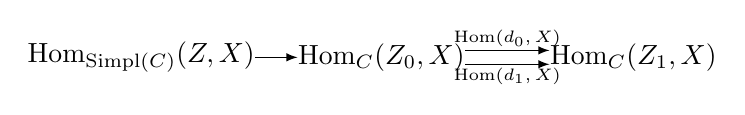
\begin{tikzpicture}[baseline=(b.base),>=latex]
    \node[inner sep=0pt] (a) at (0,0)
      {$\operatorname{Hom}_{\operatorname{Simpl}(C)}(Z,X)$};
    \node[inner sep=0pt] (b) at (3.05,0)
      {$\operatorname{Hom}_{C}(Z_0,X)$};
    \node[inner sep=0pt] (c) at (6.25,0)
      {$\operatorname{Hom}_{C}(Z_1,X)$};
    \draw[->] (a) -- (b);
    \draw[->]
      ([yshift=2.5bp]b.east) --
      node[above,inner sep=1bp,font=\fontsize{5.7}{6.4}\selectfont]
        {$\operatorname{Hom}(d_0,X)$}
      ([yshift=2.5bp]c.west);
    \draw[->]
      ([yshift=-2.5bp]b.east) --
      node[below,inner sep=1bp,font=\fontsize{5.7}{6.4}\selectfont]
        {$\operatorname{Hom}(d_1,X)$}
      ([yshift=-2.5bp]c.west);
  \end{tikzpicture}%
}

% Native-TeX homotopy diagrams from LNM 239, physical p.21 / printed p.3.
\newcommand{\IllusieHomotopyTriangle}{%
  \begin{center}
  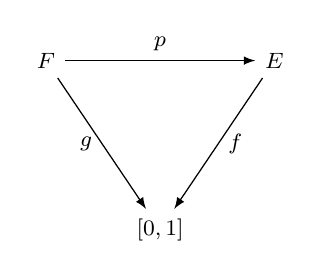
\begin{tikzpicture}[
    >=latex,
    line width=0.45pt,
    every node/.style={font=\rmfamily\fontsize{8}{9}\selectfont}
  ]
    \node (F) at (-1.45,1.0) {$F$};
    \node (E) at (1.45,1.0) {$E$};
    \node (I) at (0,-1.15) {$[0,1]$};
    \draw[->] (F) -- node[above] {$p$} (E);
    \draw[->] (F) -- node[left] {$g$} (I);
    \draw[->] (E) -- node[right] {$f$} (I);
  \end{tikzpicture}
  \end{center}%
}

\newcommand{\IllusieHomotopySquare}{%
  \begin{center}
  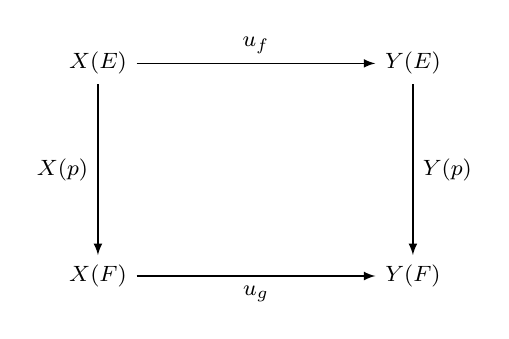
\begin{tikzpicture}[
    >=latex,
    line width=0.45pt,
    every node/.style={font=\rmfamily\fontsize{8}{9}\selectfont}
  ]
    \node (XE) at (-2.0,1.35) {$X(E)$};
    \node (YE) at (2.0,1.35) {$Y(E)$};
    \node (XF) at (-2.0,-1.35) {$X(F)$};
    \node (YF) at (2.0,-1.35) {$Y(F)$};
    \draw[->] (XE) -- node[above] {$u_f$} (YE);
    \draw[->] (XE) -- node[left] {$X(p)$} (XF);
    \draw[->] (YE) -- node[right] {$Y(p)$} (YF);
    \draw[->] (XF) -- node[below] {$u_g$} (YF);
  \end{tikzpicture}
  \end{center}%
}

% Native-TeX transitivity triangle from LNM 239, physical p.12 / Roman X.
\newcommand{\IllusieTransitivityTriangle}{%
  \begin{center}
  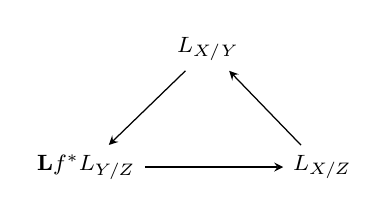
\begin{tikzpicture}[
    >=stealth,
    line width=0.45pt,
    every node/.style={font=\rmfamily\fontsize{8.15}{9}\selectfont}
  ]
    \node (xy) at (0,1.05) {$L_{X/Y}$};
    \node (fyz) at (-1.55,-0.45) {$\mathbf L f^{*}L_{Y/Z}$};
    \node (xz) at (1.45,-0.45) {$L_{X/Z}$};
    \draw[->] (xy) -- (fyz);
    \draw[->] (fyz) -- (xz);
    \draw[->] (xz) -- (xy);
  \end{tikzpicture}
  \end{center}%
}

% Native chapter-dependency guide from LNM 239 physical p.17 / Roman XV.
\newcommand{\IllusieChapterGuide}{%
  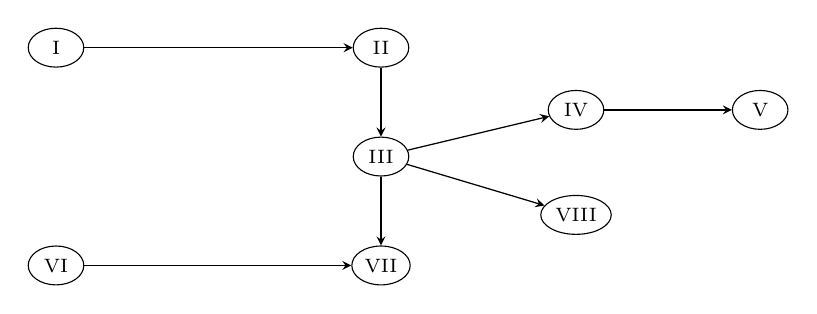
\begin{tikzpicture}[
    x=39bp,y=28bp,>=stealth,
    guide node/.style={draw,ellipse,minimum width=20bp,minimum height=14bp,
      inner sep=1.5bp,font=\fontsize{7}{7}\selectfont},
    guide arrow/.style={->,line width=0.45pt}
  ]
    \node[guide node] (I) at (0,2.8) {I};
    \node[guide node] (II) at (3,2.8) {II};
    \node[guide node] (III) at (3,1.4) {III};
    \node[guide node] (IV) at (4.8,2.0) {IV};
    \node[guide node] (V) at (6.5,2.0) {V};
    \node[guide node] (VIII) at (4.8,0.65) {VIII};
    \node[guide node] (VII) at (3,0) {VII};
    \node[guide node] (VI) at (0,0) {VI};
    \draw[guide arrow] (I) -- (II);
    \draw[guide arrow] (II) -- (III);
    \draw[guide arrow] (III) -- (IV);
    \draw[guide arrow] (IV) -- (V);
    \draw[guide arrow] (III) -- (VIII);
    \draw[guide arrow] (III) -- (VII);
    \draw[guide arrow] (VI) -- (VII);
  \end{tikzpicture}%
}


\newcommand{\IllusieVolumeOneCover}[1]{%
  \phantomsection\hypertarget{illusie:I:cover}{}%
  \begin{tikzpicture}[remember picture,overlay]
    \fill[illusiecover] (current page.south west) rectangle (current page.north east);
    \fill[black]
      ($(current page.north west)+(0,-0.01\paperheight)$)
      rectangle
      ($(current page.north east)+(0,-0.18\paperheight)$);
    \node[
      anchor=north west,
      align=left,
      text=illusiecover,
      font=\sffamily\fontsize{29}{30}\selectfont
    ] at ($(current page.north west)+(0.245\paperwidth,-0.020\paperheight)$)
      {Lecture Notes in\\Mathematics};
    \node[
      anchor=north west,
      align=left,
      text=illusiecover,
      font=\sffamily\fontsize{8.2}{10}\selectfont
    ] at ($(current page.north west)+(0.247\paperwidth,-0.126\paperheight)$)
      {A collection of informal reports and seminars\\
       Edited by A. Dold, Heidelberg and B. Eckmann, Z\"urich};
    \node[
      anchor=west,
      font=\sffamily\fontsize{28}{29}\selectfont
    ] at ($(current page.west)+(0.245\paperwidth,0.155\paperheight)$) {239};
    \draw[line width=0.55pt]
      ($(current page.west)+(0,0.105\paperheight)$) --
      ($(current page.east)+(0,0.105\paperheight)$);
    \node[
      anchor=west,
      font=\sffamily\fontsize{29}{30}\selectfont
    ] at ($(current page.west)+(0.245\paperwidth,0.035\paperheight)$)
      {Luc Illusie};
    \node[
      anchor=west,
      align=left,
      font=\sffamily\fontsize{29}{32}\selectfont
    ] at ($(current page.west)+(0.245\paperwidth,-0.205\paperheight)$)
      {#1};
    \draw[line width=0.55pt]
      ($(current page.south west)+(0,0.205\paperheight)$) --
      ($(current page.south east)+(0,0.205\paperheight)$);
    \node[anchor=west] at
      ($(current page.south west)+(0.25\paperwidth,0.145\paperheight)$)
      {\IllusieSpringerMark};
    \node[
      anchor=north west,
      align=left,
      font=\sffamily\fontsize{20}{22}\selectfont
    ] at ($(current page.south west)+(0.245\paperwidth,0.115\paperheight)$)
      {Springer-Verlag\\Berlin · Heidelberg · New York};
  \end{tikzpicture}%
  \mbox{}\vfill\clearpage
}

% Public-edition cover: author and work only. The source-cover reconstruction
% above remains available to the internal diplomatic witness, but the French
% and English editions deliberately carry no LNM or publisher branding.
\newcommand{\IllusieVolumeOneEditionCover}[1]{%
  \phantomsection\hypertarget{illusie:I:cover}{}%
  \begin{tikzpicture}[remember picture,overlay]
    \fill[illusieeditionpaper]
      (current page.south west) rectangle (current page.north east);
    \fill[illusieeditionaccent]
      ($(current page.north west)+(0,-0.115\paperheight)$)
      rectangle
      ($(current page.north west)+(0.030\paperwidth,-0.885\paperheight)$);
    \draw[illusieeditionink,line width=0.8pt]
      ($(current page.north west)+(0.125\paperwidth,-0.305\paperheight)$) --
      ($(current page.north east)+(-0.125\paperwidth,-0.305\paperheight)$);
    \node[
      anchor=south west,
      text=illusieeditionink,
      font=\sffamily\fontsize{24}{26}\selectfont
    ] at ($(current page.north west)+(0.125\paperwidth,-0.272\paperheight)$)
      {Luc Illusie};
    \node[
      anchor=north west,
      align=left,
      text=illusieeditionink,
      text width=0.73\paperwidth,
      font=\sffamily\fontsize{31}{35}\selectfont
    ] at ($(current page.north west)+(0.125\paperwidth,-0.365\paperheight)$)
      {#1};
  \end{tikzpicture}%
  \mbox{}\vfill\clearpage
}
